%% Version: 0.6 (03.01.2019)

%% Choose language: english or german
%% Choose Thesis type: seminar, bachelor, master, phd, techreport
%% Use 'declaration' parameter if you want to generate declaration page
%% Use 'final' to disable Todo-notes from final version without deleting each one of them
\documentclass[english,master]{KITthesis}

%% ---------------------------------
%% | Information about the thesis  |
%% ---------------------------------
\title{Pose Estimation for Industrial Robots\\
via Transfer Learning from Sim to Real}
\titleotherlanguage{Mein Titel\\
ist lang}

\author{Zhuoyi Han}
\address{Bernhardstr.11}
\city{76131 Karlsruhe}
\email{uxehr@studen.kit.edu}

\keywords{Keywords, of, my, Thesis}
\keywordsotherlanguge{Die, Stichw\"orter, f\"ur, meine, Arbeit}

%% Study program or a seminar/subject
\studyprogram{Intelligente Industrieroboter}

%% Name of your institute (Default: IAR-IPR)
% \institute{}
%% Name of your faculty (Default: KIT-Fakultät für Informatik
% \KITfaculty{}
%% Address of your institute (Default: Engler-Bunte-Ring 8)
% \instituteaddress{}
%% Insitute City (Default: 76131 Karlsruhe)
% \institutecity{}

\reviewerone{Prof. Dr.-Ing. Torsten Kröger}
\reviewertwo{Prof. Dr.-Ing. habil. Björn Hein}
%
% %% The advisors are PhDs or Postdocs
\advisorone{M.Sc. Yongzhou Zhang}
% %% The second advisor can be omitted
%\advisortwo{M.Sc. D}
%
% %% Please enter the start end end time of your thesis
\editingtime{11. November 2018}{31. April 2019}

%% --------------------------------
%% | Settings for word separation |
%% --------------------------------
% Help for separation:
% In german package the following hints are additionally available:
% "- = Additional separation
% "| = Suppress ligation and possible separation (e.g. Schaf"|fell)
% "~ = Hyphenation without separation (e.g. bergauf und "~ab)
% "= = Hyphenation with separation before and after
% "" = Separation without a hyphenation (e.g. und/""oder)

% Describe separation hints here:
\hyphenation{
% Pro-to-koll-in-stan-zen
% Ma-na-ge-ment  Netz-werk-ele-men-ten
% Netz-werk Netz-werk-re-ser-vie-rung
% Netz-werk-adap-ter Fein-ju-stier-ung
% Da-ten-strom-spe-zi-fi-ka-tion Pa-ket-rumpf
% Kon-troll-in-stanz
}

%%
%% --------------------
%% |   Bibliography   |
%% --------------------
\newcommand{\mybibliographyfiles}{Bibliography/ipr_articles,Bibliography/kit_template_example_bibliography,Bibliography/my_thesis_bibliography}


%% --------------------
%% |     Acronyms     |
%% --------------------
\newacronym{ipr}{IAR-IPR}{Institute for Anthropomatics and Robotics - Intelligent Process Control and Robotics}

%% --------------------
%% |     Glossary     |
%% --------------------
\newglossaryentry{robot}
{
    name=robot,
    description={The robot developed in this work.}
}


%% ------------------------
%% |    Including files   |
%% ------------------------
% Only files listed here will be included!
% Userful command for partially translating the document (for bug-fixing e.g.)
% \includeonly{%
% Content/0-Declaration,
% Content/0-Abstract_EN,
% Content/0-Abstract_DE,
% Content/1-Introduction,
% Content/2-State-of-the-art,
% Content/3-Methods,
% Content/4-Concept,
% Content/5-Implementation,
% Content/6-Results,
% Content/7-Discussion,
% Content/8-Conclusion,
% Content/11-Appendix,
% }

\settitle
%%%%%%%%%%%%%%%%%%%%%%%%%%%%%%%%%
%% Here, main documents begins %%
%%%%%%%%%%%%%%%%%%%%%%%%%%%%%%%%%
\begin{document}
%% Uncomment this to use only first authors name in bibliography
% \bstctlcite{BSTcontrol}

%% Set PDF metadata
\setpdf

%% Title Page
\includetitle

% TODO: Remove this from final version
\includelistoftodos

\includedeclaration

\includeacknowledgments

%% ----------------
%% |   Abstract   |
%% ----------------
%% An abstract both in English
%% and German is mandatory.
%%
%% The text is included from the following files:
%% - Content/0-Abstract_EN
%% - Content/0-Abstract_DE
\includeabstract

%% ------------------------
%% |   Table of Contents  |
%% ------------------------
\inculdetableofcontents

\makenomenclature

%% -----------------
%% |   Main part   |
%% -----------------
\setmainpart

%% ==============================
% Part is used only in PhD thesis
\part{The challenges}
\chapter{\iflanguage{ngerman}{Einleitung}{Introduction}}
\label{sec:Introduction}
%% ==============================
Robot learning has attracted an increasing amount of attention in recent years.  With the development of technology robots are required to conduct complex tasks and tackle unforeseen circumstances. Giving robots the ability to learn is paramount for ensuring the success of future robotic system. Perceiving and processing information from environment are particularly important for robot learning.

Pose estimation of an object from pixels is a well-studied problem of perceiving task in robotics. Pose estimation can be achieved by a variety of methods, including the approach based on image. Estimation from camera pixels is attractive due to the low cost of cameras and the rich data they provide, but challenging because it involves processing high-dimensional input data. Recent work has shown that supervised learning with deep neural networks is a powerful tool for learning generalizable representations from high-dimensional inputs \cite{lecun2015yoshua}, and state-of- the-art methods employ complex, hand-engineered image processing pipelines (e.g., \cite{collet2011moped}, \cite{tang2012textured}). This work is a first step toward the goal of using deep learning to improve the accuracy of object detection pipelines. But deep learning relies on a large amount of labeled data. Labeled data is difficult to obtain in the real world for precise robotic manipulation behaviors, but it is easy to generate in a physics simulator. So the concept of transfer learning was proposed. The main idea is to realize the learning process in simulation and then transfer the knowledge to the robot in real world, which is called \textit{sim-to-real}.

Learning in simulation is especially promising for building on recent results using deep reinforcement learning to achieve human-level performance on tasks like Atari \cite{mnih2015human} and robotic control \cite{levine2016end}. However, discrepancies between physics simulators and the real world make transferring behaviors from simulation challenging. Some recent work has received good results on the overcoming the reality gap. Robustness from sim to real can be improved by injecting noise \cite{su2015render}, using domain randomization \cite{tobin2017domain}, domain adaptation \cite{sun2014virtual}, Although not explicitly using real-world data for training, these methods have been shown effective to increase the success rate of sim-to-real transfer

\section{Aim of the Thesis}
The final goal of the thesis is combined with the above methods to optimize the pose estimation via transfer learning, for improving the robustness of the detector from sim to real. And further optimization will be performed for higher estimation accuracy. For performing robotic learning in a physics simulator, the simulation scene is built based on Unity3D rendering engine. The deep neural network models were then built and optimized to obtain a accurate object detector. To analyze the effects of different rendering conditions on accuracy and robustness of detector, various simulation scenes were built. Finally, the estimation accuracy is further improved by using a dual-camera system.

In order to achieve the final goal, the following sub-goals are pursued:
\begin{itemize}
	\item Set up a simulation environment for the experiment with different function modules, which can achieve various rendering effects.
	\item Design a deep neural network model for the task and optimize its performance.
	\item Compare the effects of different rendering conditions on prediction accuracy and robustness.
	\item Further optimization through dual-camera system. 
	\item Evaluate the performance of detector by performing robot grasping experiment.
\end{itemize}

\section{Contributions}
In this thesis, in order to optimize the pose estimation based on sim-to-real transfer, a complete pipeline has been built, which starts from building a simulation environment to detector optimization and finally to robotic experiments. The main contributions are:

\begin{itemize}
	\item The pipeline laid the foundation for further research based on transfer learning. The research focusing on multi-objects estimation and robot control can be extended on our pipeline.
	\item The simulation environment in the experiment can be used for other deep learning learning tasks. The rendering environment consists of different functional modules, which can be used for other projects by modifying the functions.
	\item Verification of the feasibility of transfer learning for our pose estimation task.
\end{itemize}

\section{Outline}
According to the stated main goals, the remainder of this thesis is structured as outlined in the following:

Chapter 2 gives an overview of the state-of-the-art. The related works in object detection and pose estimation in robotics are presented. The it describe the methods for overcoming  the reality gap, e.g. domain adaptation and domain randomization.

Chapter3 introduces the technical background of thesis. Section 3.1 gives the basic knowledge of interaction interface and scene rendering in Unity3D. Section 3.2 describes the principle and structure of the deep neural network. Several well-known convolutional neural network models are introduced in section 3.3.

The pipeline architecture design and functionality explanation of different modules is presented in Chapter 4. Section 4.1 describes the structure of overall pipeline. Section 4.2 describes the different function modules of simulation environment. The structure design and training process are introduces in section 4.3. Finally, the evaluation module and the data collection process in real world are presented.

Chapter5 introduces the experimental process and results analysis. Section 5.1 describes the scene settings in both real world and simulation environment. Model optimization and rendering scene optimization are mentioned in section 5.2 and 5.3. In Section 5.4 the dual-camera system was used to optimize the estimation accuracy. Finally, the robotic experiments are introduced in section 5.5.

In Chapter 6, conclusions are drawn and potential future works are presented.

%% ==============================
\chapter{\iflanguage{ngerman}{Stand der Wissenschenschaft und Technik}{State of the art}}
\label{sec:state_of_the_art}
%% ==============================
This chapter describes the current state of the art of our work. We did a comprehensive literature research on the topic of object detection and pose estimation for robotics and different approaches to bridge the reality gab, which means the barrier to using simulated data on real robots. We describe the results of this literature research in the following sections. In Section 2.1, we reviews different methods which used on object detection and pose estimation for robotics. In Section 2.2, we focus on the approach domain randomization to bridge the reality gap. In Section 2.3, we give an overview of the domain adaptation which are used for training models to a previously unseen target domain.  Section 2.4 gives a summary to the these approaches.

\section{Object detection and pose estimation for robotics}
Object detection and pose estimation for robotics is a well-studied problem in the literature. Recent approaches typically involve offline construction or learning of a 3D model of objects in the scene (e.g., a full 3D mesh model \cite{tang2012textured} or a 3D metric feature representation \cite{collet2011moped}). At test time, features from the test data (e.g., Scale-Invariant Feature Transform [SIFT] features \cite{gordon2006and} or color co-occurrence histograms \cite{ekvall2005object} are matched with the 3D models (or features from the 3D models). For example, a black-box nonlinear optimization algorithm can be used to minimize the re-projection error of the SIFT points from the object model and the 2D points in the test image \cite{collet2009object}. Most successful approaches rely on using multiple camera frames \cite{collet2010efficient} or depth information \cite{tang2012textured}. There has also been some success with only monocular camera images \cite{collet2009object}.

These traditional approaches require less extensive training and take advantage of richer sensory data, allowing them to detect the full 3D pose of objects (position and orientation) without any assumptions about the location or size of the surface on which the objects are placed. However, in this thesis we aims to avoids the challenging problem of 3D reconstruction, and employs a simple, easy to implement deep learning-based pipeline that may scale better to more challenging problems.

\section{Domain Randomization}
Domain randomization is a complementary class of techniques for adaptation that is particularly well suited for simulation. With domain randomization, discrepancies between the source and target domains are modeled as variability in the source domain. Randomization in the visual domain has been used to directly transfer vision-based policies from simulation to the real world without requiring real images during training \cite{sadeghi2016cad2rl}, \cite{tobin2017domain}. 

Sadeghi and Levine \cite{sadeghi2016cad2rl} trained vision-based controllers for a quadrotor using only synthetically rendered scenes, and Tobin et al. \cite{tobin2017domain} demonstrated transferring image-based object detectors. Unlike previous methods, which sought to bridge the reality gap with high fidelity rendering \cite{james20163d}, their systems used only low fidelity rendering and modeled differences in visual appearance by randomizing scene properties such as lighting, textures, and camera placement. The approach in \cite{tobin2017domain} does not rely on precise camera information or calibration, instead randomizing the position, orientation, and field of view of the camera in the simulator. Whereas approach in \cite{sadeghi2016cad2rl} chooses textures from a dataset of around 200 pre-generated materials, most of which are realistic, the approach in \cite{tobin2017domain} use only non-realistic textures created by a simple random generation process. Figure 2.1 shows the rendering scene by Tobin et al. \cite{tobin2017domain} in their work.
\begin{figure}[h]
	\centering
	\includegraphics{Figures/Section2_Tobin}
	\caption{Rendered low-fidelity images with random camera positions, lighting conditions, and non-realistic textures in \cite{tobin2017domain} }
	\label{fig: tobin work}
\end{figure}

\section{Domain adaptation}
Another way to cross the reality gap is to learn from both simulation and real-world data. The computer vision community has devoted significant study to the problem of adapting vision-based models trained in a source domain to a previously unseen target domain (see, e.g., \cite{hoffman2014lsda}, \cite{hoffman2013efficient}, \cite{long2015learning}). A variety of approaches have been proposed, including re-training the model in the target domain (e.g., \cite{yosinski2014transferable}),  adapting the weights of the model based on the statistics of the source and target domains (e.g., \cite{li2016revisiting}), learning invariant features between domains (e.g., \cite{tzeng2014deep}), and learning a mapping from the target domain to the source domain (e.g., \cite{taigman2016unsupervised}). Researchers in the reinforcement learning community have also studied the problem of domain adaptation by learning invariant feature representations \cite{gupta2017learning}, adapting pretrained networks \cite{rusu2016progressive}, and other methods. See \cite{gupta2017learning} for a more complete treatment of domain adaptation in the reinforcement learning literature.

It is often faster to fine-tune a controller learned in simulation than to learn from scratch in the real world \cite{cutler2015efficient, kolter2007learning}. In \cite{ghadirzadeh2017deep}, the authors use a variational autoencoder trained on simulated data to encode trajectories of motor outputs corresponding to a desired behavior type (e.g., reaching, grasping) as a low-dimensional latent code. A policy is learned on real data mapping features to distributions over latent codes. The learned policy overcomes the reality gap by choosing latent codes that correspond to the desired physical behavior via exploration.

Domain adaptation has also been applied to robotic vision. Rusu et al. \cite{rusu2016sim} explore using the progressive network architecture to adapt a model that is pretrained on simulated pixels, and find it has better sample efficiency than fine-tuning or training in the real-world alone. In \cite{tzeng2015adapting}, the authors explore learning a correspondence between domains that allows the real images to be mapped into a space understood by the model. While both of the preceding approaches require reward functions or labeled data, which can be difficult to obtain in the real world, Mitash and collaborators \cite{mitash2017self} explore pretraining an object detector using realistic rendered images with randomized lighting from 3D models to bootstrap an automated learning process that does not require manually labeling data and uses only around 500 real-world samples.

\section{Overcoming the reality gap}
Previous work on leveraging simulated data for physical robotic experiments explored several strategies for bridging the reality gap. We summarize it as follows:

One type of approach is to make the simulator closely match the physical reality by performing system identification and using high-quality rendering. Though using realistic RGB rendering alone has had limited success for transferring to real robotic tasks \cite{james20163d}, incorporating realistic simulation of depth information can allow models trained on rendered images to transfer reasonably well to the real world \cite{planche2017depthsynth}. Combining data from high-quality simulators with other approaches like fine-tuning can also reduce the number of labeled samples required in the real world \cite{richter2016playing}. Unlike these approaches, the other type allows the use of low-quality renderers optimized for speed and not carefully matched to real-world textures, lighting, and scene configurations. And it requires no additional training on real-world data \cite{tobin2017domain}.

For a better result by overcoming the reality gap, the two types of approaches can be combined.






% %% ==============================
% Part is used only in PhD thesis
\part{The ideas}
\chapter{\iflanguage{ngerman}{Methoden}{Methods}}
\label{sec:methods}
%% ==============================
\section{title}
\dots



%% ==============================
\chapter{\iflanguage{ngerman}{Konzept}{Technogical Fundations}}
\label{sec:Technogical Fundations}
%% ==============================
This chapter introduces technological foundations fundamental for this thesis, which includes methods, models and tools that are used later in the thesis. The first section focus on the basic principle of Unity3D, which is used to build simulation environment for generating synthetic images. Then the second section shortly explain the essential knowledge of deep learning, especially convolution neural network(CNN), which used by modeling to recognize objects and predict the 3D-pose of them. Section 2.2 give an overview of the Kreas/Tensorflow framework, which will be used for training the CNN-model. Section 2.3 shows how to build a shallow neural network model in Keras and train it.

\section{Unity3D background}
Unity is a cross-platform game engine developed by Unity Technologies. Due to the motivation of transfer learning from simulation to real environment, a simulation scene in virtual environment need to be built and large numbers of synthetic image data of it are requisite. The unity engine gives users the ability to create virtual objects in 3D and offers a primary scripting API in C\# to render images that are needed in this research. All these features shows that Unity is suitable for rendering requests and can simplify the works during modeling. 
\subsection{User interface}
Unity provides a basic graphical interface to build the simulation environment, which includes five basic windows. 
\begin{itemize}
	\item The Scene View: where user work with game objects, including models, lights and colliders, to construct the user's scenes. 
	\item The Game View: where user can preview and play simulation scene as a work in progress as user develop it.
	\item The hierarchy window: All of the game objects in the open scenes are listed by the hierarchy window in hierarchical order.
	\item The project window: where user imports, stores and edits the Asset files. 
	\item The inspector window: It is context sensitive and displays all the properties of any selected game object, asset or setting.
\end{itemize} 
All the modeling works can be done in the graphical user interface. A general method of modeling are divided into 4 steps. Firstly a new default model needs to be created in Unity or imported from other 3D modeling software. This new model will appear in hierarchy window with other existent objects. Here the hierarchical relations can be adjusted. Secondly the dimensions and positions of new created model can be modified in inspector window, and new components (e.g. C\# scripts, Mesh Renderer, etc.) can be added into the model. Then in scene window a arbitrary perspective could be set, and according to the local coordinate system the position relationship among different objects can be adjusted. Finally when all items are correctly set and all needed components are added on them, the simulation scene can be played and the progress can be monitored in game view window in real time.
\subsection{Coordinate system in Unity}
The world coordinate system is left handed (as Direct X) where x positive axis is right, y positive is up and z is positive into the screen.\\
\begin{figure}[h]
	\centering
	\captionsetup{justification=centering}
	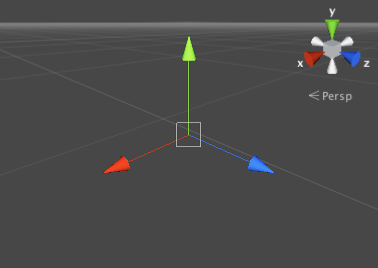
\includegraphics{{Figures/Section3_CoordinateSystem.png}}
	\caption{Coordinate system in Unity}
	\label{fig: Coordinate unity}
\end{figure}\\
Screen coordinate system is bottom-up: (0,0) at bottom-left corner and (pixelWidth-1,pixelHeight-1) at right-top; x axis is positive right and y is positive up. The z position is in world units from the camera.\\
Viewport coordinate system is normalized and relative to the camera, so the bottom-left point is (0,0), the top-right is (1,1). The z position is in world units from the camera.\\
Finally UI coordinate system is top-down: the y coordinate varies from zero at the top edge of the window to a maximum at the bottom edge of the window. The upper-left point is (0,0); the bottom-right is (1,1).\\
There are many functions to convert between all these different coordinate systems
\subsection{Basic concepts in scene}
To build a basic scene in Unity 3D, some important core concepts need to be known. which include Game Object, Component, Script and etc. They form the main basic elements of unity and should be added into the scene to realize the needed functions and effects. Normally the Component and Script are sub-element of the Game Object.\\
\begin{itemize}
	\item Scenes: Scenes contain the objects of simulation project. They can be used to create a main menu, individual levels, and anything else. Each unique Scene file is a unique level. In each Scene, the environments, obstacles, decorations will be placed, and the project are designed and built in pieces.\\
	A new Unity project will show a new Scene. The scene will be empty except for default objects- either an orthographic camera, or a  perspective camera and a directional light. 
	\item GameObjects: The GameObject is the most important concept in the Unity Editor.\\
	Every object in project is a GameObject. This means that everything which can be thought of to be in the project has to be a GameObject. However, a GameObject can't do anything on its own; The properties need to be given before it can become a character, an environment, or a special effect.\\
	A GameObject is a container; pieces are added to the GameObject container to make it into a character, a light, or whatever needed in project. Each added piece is called a component.\\
	Depending on what kind of object need to be created, different combinations of components can be added to a GameObject. A GameObject could be thought of as an empty cooking pot, and components are different ingredients that make up the recipe of project.  
	\item Component: Components are the nuts \& bolts of objects and behaviors in a game. They are the functional pieces of every GameObject.\\
	A GameObject is a container for many different Components. By default, all GameObjects automatically have a Transform Component. This is because the Transform dictates where the GameObject is located, and how it is rotated and scaled. Without a Transform Component, the GameObject wouldn't have a location in the word.
	\item Script: Scripting is an essential ingredient in all projects. They can be used to create graphical effects, control the physical behavior of objects and even implement a custom automatic system in the project. In next subsection, basic knowledge of scripting will be introduced to show how the script runs in unity and which basic functions are included in it. 
\end{itemize}
\subsection{Basic knowledge of script}
Unity supports the C\# programming language, which is an industry-standard language similar to Java or C++.\\
A script makes its connection with the internal workings of Unity by implementing a class which derives from the built-in class called MonoBehaviour. A class is like a kind of blueprint for creating a new Component type that can be attached to GameObjects. The core elements to realize different effects are the Event Functions. A script in Unity is not like the traditional idea of a program where the code runs continuously in a loop until it completes its task. Instead, Unity passes control to a script intermittently by calling certain functions that are declared within it. Once a function has finished executing, control is passed back to Unity. These functions are known as event functions since they are activated by Unity in response to events that occur during gameplay. Unity uses a naming scheme to identify which function to call for a particular event. There are four basic types of events:
\begin{itemize}
	\item Regular Update Events: 
	\begin{enumerate}
		\item Update function: The Update function is the main place for making changes to position, state and behavior of objects in the scene just before each frame is rendered. Update is called before the frame is rendered and also before animations are calculated.
		\item FixedUpdate function: The physics engine also update in discrete time steps in a similar way to the frame rendering. A separate event function called FixedUpdate is called just before each physics update.
		\item LateUpdate function: It is also useful sometimes to be able to make additional changes at a point after the Update and FixedUpdate functions have been called for all objects in the scene and fter all animations have been calculated.
	\end{enumerate}
	\item Initialization Events:
	\begin{enumerate}
		\item Start function: It is called before the first frame or physics update on an object.
		\item Awake function: The Awake function is called for each object in the scene at the time when the scene loads. All the Awakes will have finished before the first Start is called. This means that code in a Start function can make use of other initializations previously carried out in the Awake phase.
	\end{enumerate}
	\item GUI event: Unity has a system for rendering GUI controls over the main action in the scene and responding to clicks on these controls. This code is handled somewhat differently from the normal frame update and so it should be placed in the OnGUI function, which will be called periodically.
	\item Physics events: The physics engine will report collisions against an object by calling event functions on the object's script. 		
\end{itemize}
\begin{figure}[h]
	\centering
	\captionsetup{justification=centering}
	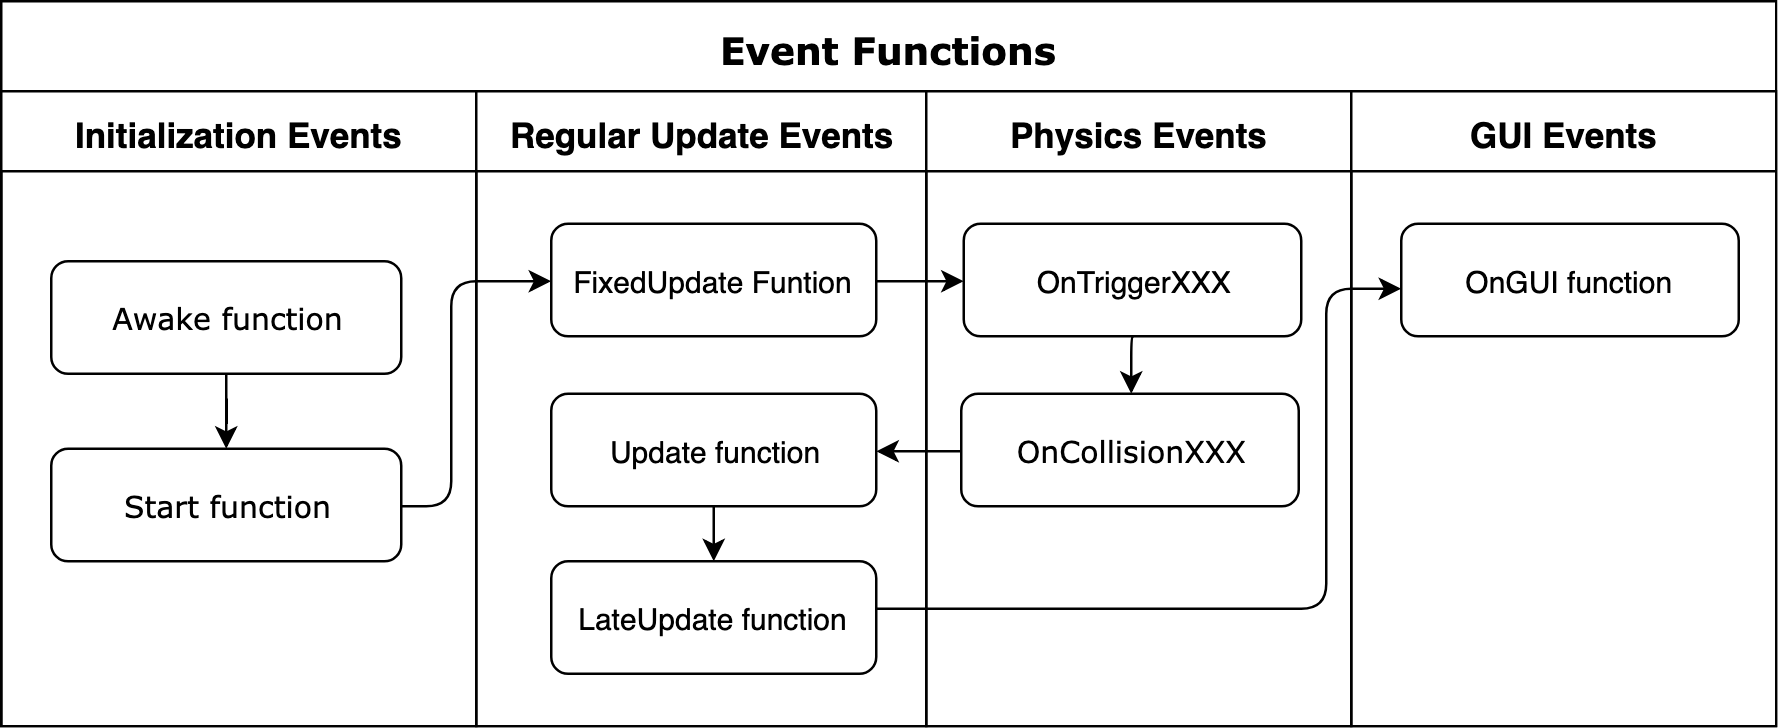
\includegraphics[width=\textwidth]{Figures/Section3_Eventfunction.png}
	\caption{Event function and execution order in Unity}
	\label{fig: event_function}
\end{figure}

\section{Neural network and Deep Learning}
In this section a introduction to neural network and deep learning are presented with the aim of enabling the reader to build up a precise understanding of the concepts and ideas as well as of the thesis' context.\\
The simplest definition of a neural network, more properly referred to as an 'artificial' neural network (ANN), is provided by the inventor of one of the first neuro-computers, Dr.Robert Hecht-Nielsen. "It is a computing system made up of a number of simple, highly interconnected processing elements, which process information by their dynamic state response to external inputs."\\
ANNs are processing devices (algorithms or actual hardware) that are highly simplified technical implementations for modeling information processing in the brain and nervous system.
\subsection{Biological motivation and connections}
The basic computational unit of the brain is a neuron. Approximately 86 billion neurons can be found in the human nervous system and they are connected with approximately $10^14$-$10^15$ synapses. The diagram below shows a cartoon drawing of a biological neuron and a common mathematical model.
\begin{figure}[h]
	
	\begin{subfigure}{0.5\textwidth}
		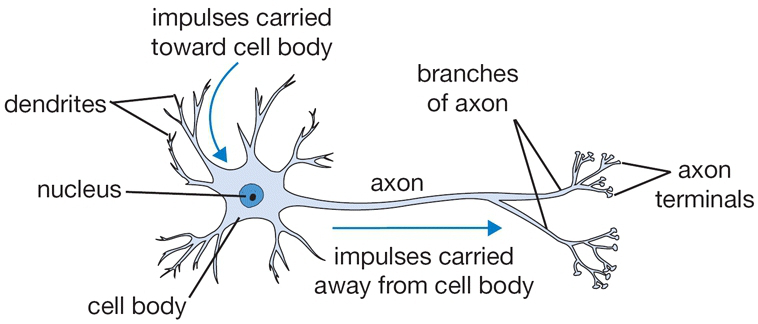
\includegraphics[width=0.9\linewidth, height=4cm]{Figures/Section3_NeuroStructure.png} 
		\captionsetup{justification=centering}
		\caption{Biological Neuron}
		\label{fig:Bio neuron}
	\end{subfigure}
	\begin{subfigure}{0.5\textwidth}
			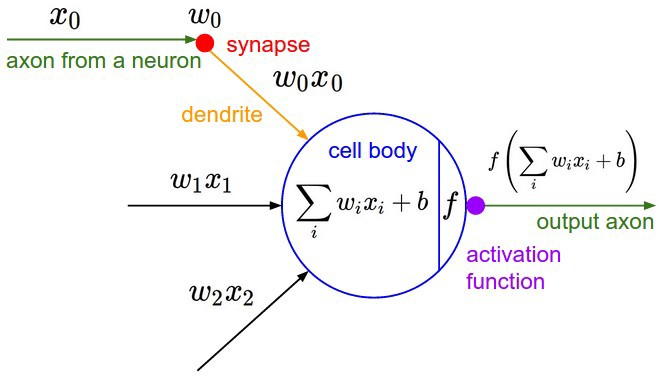
\includegraphics[width=0.9\linewidth, height=4cm]{Figures/Section3_NeuroMathe.jpeg}
			\captionsetup{justification=centering}
			\caption{mathematical model of neuron}
			\label{fig:mathe neuron}
	\end{subfigure}
\captionsetup{justification=centering}
\caption{Basic Neuron Unit}
\label{fig:unit of a neuron}
\end{figure}
The basic unit of computation in a neural network is the neuron, often called a node or unit. It receives input from some other nodes, or form an external source and computes an output. Each input has an associated weight (w), which is assigned on the basis
\subsection{Neural Network Architecture}
\subsection{Commonly used activation functions}
\subsection{Gradient Descent for Neural Networks}
\subsection{Forward Propagation and Back Propagation}
\subsection{title}

%% ==============================
% Part is used only in PhD thesis
\part{The Implementation}
\chapter{\iflanguage{ngerman}{Implementierung}{Implementation}}
\label{sec:implementation}
%% ==============================

\dots
\missingfigure{Please add some figures}



%% ==============================
\chapter{\iflanguage{ngerman}{Ergebnisse}{Results}}
\label{sec:results}
%% ==============================

\dots

%% ==============================
% Part is used only in PhD thesis
\part{The Evaluation}
\chapter{\iflanguage{ngerman}{Diskussion}{Discussion}}
\label{sec:discussion}
%% ==============================

\dots



%% ==============================
\chapter{\iflanguage{ngerman}{Zusammensaffung und Ausblick}{Conclusion}}
\label{sec:conclusion}
%% ==============================

\dots




%% --------------------
%% |   Bibliography   |
%% --------------------
\Bibliography{\mybibliographyfiles}

%% ----------------
%% |   Appendix   |
%% ----------------
% \cleardoublepage
%% appendix.tex
%%

%% ==============================
\Appendix
\label{ch:Appendix}
%% ==============================



\section{First Appendix Section}
		\label{Anhang-Implementierung}



\begin{figure} [ht]
  \centering
   ein Bild
  \caption{A figure}
  \label{fig:BPMNBeispiela}
\end{figure}


\dots





% Remove if needed
%% -----------------------------
%% |   List of Figures/Tables  |
%% -----------------------------
\includeglossaries
\inculdelistoffigures
\inculdelistoftables
\inculdelistoflistings
\inculdelistofalgoritms

%% --------------------
%% |   MyBib Entry    |
%% --------------------
\addmybibentry

%% --------------------------------
%% |   How to use this document   |
%% --------------------------------
\includehowtouse

\end{document}
